\documentclass[a4paper, 11pt]{book}
\usepackage{/home/nora/Documents/Enseignement/Prepa/bpep/fichiers_utiles/preambule}

\makeatletter
\renewcommand{\@chapapp}{Kh\^olles MPSI3 -- semaine}
\makeatother
\renewcommand\thechapter{4}

% \toggletrue{corrige}  % décommenter pour passer en mode corrigé

\begin{document}

\resetQ
\newpage

\chapter{Sujet 1\siCorrige{\!\!-- corrig\'e}}

\subimport{/home/nora/Documents/Enseignement/Prepa/bpep/exercices/TD/loi_noeuds_potentiel/}{sujet.tex}

\resetQ
\newpage

\chapter{Sujet 2\siCorrige{\!\!-- corrigé}}
\section{Pont de Wheatstone}

\QR{\begin{minipage}{0.65\linewidth}
		En électronique, on réalise régulièrement des ponts de mesure pour
		mesurer indirectement une résistance. On dispose d'un circuit comprenant
		un générateur de tension qui alimente un pont de Wheatstone composé des
		résistances $R_1$ et $R_2$. La résistance $R_i$ est inconnue, et la
		résistance $R$ est variable (il s'agit d'un potentiomètre). On fait
		évoluer $R$ jusqu'à ce que le voltmètre indique une tension nulle. Le
		pont est alors équilibré. \bigbreak

		À l'aide des lois de Kirchhoff, déterminer l'expression de la valeur de
		$R_i$ en fonction des valeurs des autres résistances lorsque le pont est
		équilibré.
	\end{minipage}
	\begin{minipage}{0.35\linewidth}
		\begin{center}
			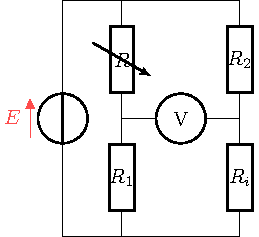
\includegraphics[width=\linewidth]{wheatstone-plain}
		\end{center}
	\end{minipage}}{
	\begin{tcbraster}[raster columns=6, raster equal height=rows]
		\begin{tcb}[raster multicolumn=2](data){Schéma}
			\begin{center}
				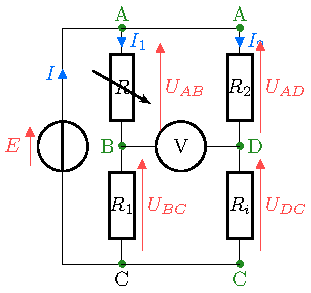
\includegraphics{wheatstone}
			\end{center}
		\end{tcb}
		\begin{tcolorbox}[blankest, raster multicolumn=1, space to=\myspace]
			\begin{tcbraster}[raster columns=1]
				\begin{tcb}*[add to natural height=\myspace](ques){Résultat attendu}

					\fontsize{10pt}{12pt}\selectfont On cherche $R_i$, ou
					$U_{DC}$ quand «~le pont est équilibré~».
				\end{tcb}
				\begin{tcb}*(tool){Outil}

					\fontsize{10pt}{12pt}\selectfont D'après l'énoncé, le pont
					est équilibré quand $V = 0$, soit quand $V_B = V_D$.

				\end{tcb}
			\end{tcbraster}
		\end{tcolorbox}
		\begin{tcb}[raster multicolumn=3](appl)'r'{Application} Si le pont est
			équilibré, alors $U_{AB} = U_{AD}$ et $U_{BC} = U_{DC}$. Or, avec le
			pont diviseur de tension, on a à la fois
			\begin{align*}
				U_{BC} & = E \frac{R_1}{R_1+R}   \\
				U_{DC} & = E \frac{R_i}{R_i+R_2}
			\end{align*}
			Donc
			\begin{align*}
				U_{BC}                                & = U_{DC}                         \\
				\Leftrightarrow \cancel{E} \frac{R_1}{R_1+R}
				                                      & = \cancel{E} \frac{R_i}{R_i+R_2} \\
				\Leftrightarrow R_1(\cancel{R_i}+R_2) & = R_i(\cancel{R_1}+R)            \\
				\Leftrightarrow \Aboxed{R_i           & = \frac{R_1R_2}{R}}
			\end{align*}
		\end{tcb}
	\end{tcbraster}
}

\resetQ
\newpage

\chapter{Sujet 4\siCorrige{\!\!-- corrigé}}
\subimport{/home/nora/Documents/Enseignement/Prepa/bpep/exercices/Colle/loi_kirchhoff_4/}{sujet.tex}

\resetQ
\newpage

\chapter{Sujet 5\siCorrige{\!\!-- corrigé}}
\subimport{/home/nora/Documents/Enseignement/Prepa/bpep/exercices/Colle/batterie_tampon/}{sujet.tex}

\resetQ
\newpage

\chapter{Sujet 6\siCorrige{\!\!-- corrigé}}

\section{Association de générateurs~: application}

\QR{Deux générateurs de tension ($E_1$, $r_1$) et ($E_2$, $r_2$) sont placés en
	parallèle l'un de l'autre. Ils alimentent une résistance $R_4$, également
	placée en parallèle sur les générateurs.
	\begin{enumerate}
		\item Dessiner le schéma normalisé de ce montage et flécher les courants
		      et les tensions.
		\item Exprimer l'intensité du courant qui circule dans $R_4$.
		\item Exprimer la tension aux bornes de $R_4$.
	\end{enumerate}}{
	\begin{tcbraster}[raster columns=2, raster equal height=rows]
		\begin{tcb}(data){Schéma}
			\begin{center}
				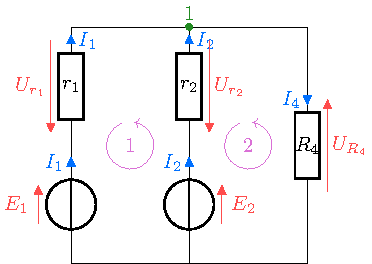
\includegraphics{assogen_parr-ldm}
			\end{center}
		\end{tcb}
		\begin{tcolorbox}[blankest, space to=\myspace]
			\begin{tcbraster}[raster columns=1]
				\begin{tcb}[add to natural height=\myspace](ques)'r'{Résultat attendu}
					On cherche $I_4$ puis $U_4 = R_4I_4$.
				\end{tcb}
				\begin{tcb}(tool)'r'{Outils}
					\begin{itemize}
						\item LdM 1~: $I_4R_4 + I_1r_1 = E_1 \quad \color{ForestGreen}(1)$~;
						\item LdM 2~: $I_4R_4 + I_2r_2 = E_2 \quad \color{ForestGreen}(2)$~;
						\item LdN 1~: $I_1 + I_2 = I_4 \quad \color{ForestGreen}(3)$.
					\end{itemize}
				\end{tcb}
			\end{tcbraster}
		\end{tcolorbox}
	\end{tcbraster}
	\begin{tcbraster}[raster columns=7, raster equal height=rows]
		\begin{tcb}[raster multicolumn=3](ror){Approche méthodique}
			Notre but est de trouver une équation contenant $I_4$ et des valeurs
			connues, c'est-à-dire tout sauf $I_1, I_2$.
			\bigbreak
			L'équation \textcolor{ForestGreen}{(1)} peut nous aider~; on peut la
			transformer en remplaçant $I_1$ par $I_4-I_2$ grâce à
			\textcolor{ForestGreen}{(3)} pour avoir une équation
			\textcolor{ForestGreen}{(4)} avec $I_4$ et $I_2$.
			\bigbreak
			Mais comme \textcolor{ForestGreen}{(2)} nous permet d'isoler $I_2$ et de
			l'exprimer en fonction de $I_4$, en injectant cette expression dans
			\textcolor{ForestGreen}{(4)} on obtient une équation entre $I_4$ et les
			éléments du circuit. Question résolue !
		\end{tcb}
		\begin{tcb}[raster multicolumn=4](appl)'r'{Application}
			Avec \textcolor{ForestGreen}{(3)} dans \textcolor{ForestGreen}{(1)}~:
			\[I_4R_4 + (I_4-I_2)r_1 = E_1 \quad \color{ForestGreen}(4)\]
			En réexprimant \textcolor{ForestGreen}{(2)}~:
			\[I_2 = (E_2 - I_4R_4)/r_2\]
			En injectant \textcolor{ForestGreen}{(2)} dans
			\textcolor{ForestGreen}{(4)}~:
			\begin{align*}
				I_4(R_4+r_1) - (E_2-I_4R_4) \frac{r_1}{\color{brandeisblue}r_2}
				 & = E_1                          \\
				\Leftrightarrow I_4(\textcolor{orange}{R_4} +
				\textcolor{red}{r_1})
				{\color{brandeisblue}r_2}
				-
				(E_2-I_4\textcolor{orange}{R_4})
				\textcolor{red}{r_1}
				 & = E_1{\color{brandeisblue}r_2} \\
				\Leftrightarrow I_4(\textcolor{red}{r_1}
				\textcolor{brandeisblue}{r_2} +
				\textcolor{red}{r_1}\textcolor{orange}{R_4} +
				\textcolor{brandeisblue}{r_2}\textcolor{orange}{R_4})
				 & = E_1r_2 +E_2r_1
			\end{align*}
			Soit
			\[\boxed{I_4 = \frac{E_1r_2 + E_2r_1}{r_1r_2+r_1R_4+r_2R_4}} \quad
				\text{et} \quad \boxed{U_{R_4} = R_4\times I_4}\]
		\end{tcb}
	\end{tcbraster}
}

\end{document}
